\documentclass{article}

\usepackage[ngerman]{babel}
\usepackage[utf8]{inputenc}
\usepackage[T1]{fontenc}
\usepackage{hyperref}
\usepackage{csquotes}
\usepackage[a4paper]{geometry}
\usepackage{graphicx}
\usepackage{float}
\usepackage{caption}

\usepackage[
    backend=biber,
    style=authoryear,
    sortlocale=de_DE,
    natbib=true,
    url=false,
    doi=false,
    sortcites=true,
    sorting=nyt,
    isbn=false,
    hyperref=true,
    backref=false,
    giveninits=false,
    eprint=false]{biblatex}
\addbibresource{../references/bibliography.bib}

\title{Ethischer Umgang mit Daten im Zusammenhang mit der KI}
\author{Max Brügger}
\date{\today}

\parskip=2em
\parindent=1em

\begin{document}

\maketitle

\begin{figure}[h]
    \centering
    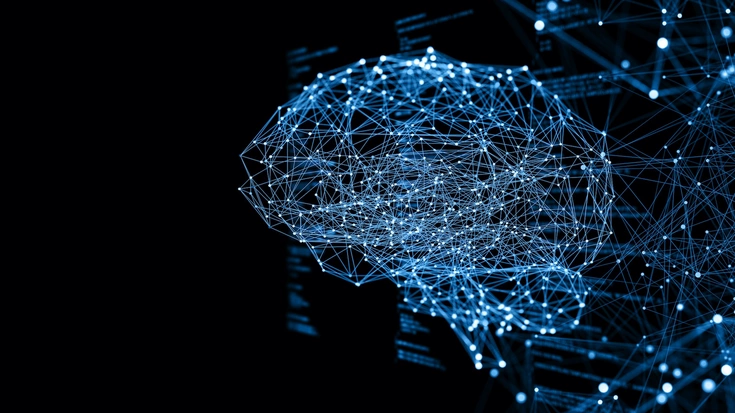
\includegraphics[width=0.5\textwidth]{brain.png}
    \caption{Ein erstes Bild}
\end{figure}

\clearpage

\tableofcontents

\clearpage


\section{Einleitung}
In dieser Arbeit befassen wir uns mit dem ethischen Umgang mit Daten im Zusammenhang mit der KI (künstliche Intelligenz). Zu diesem Thema  recherchieren wir im Internet mit KI-Programmen, erstellen Notizen und verfassen eine Arbeit zu einer Frage bezüglich der Ethik der KI, die wir uns stellen. Ich habe mich entschieden, das Thema KI in der Medizin zu beleuchten und die Chancen und Gefahren aufzuzeigen.

Um die KI  besser zu verstehen, werde ich vorab kurz die KI und ihre Einsatzgebiete definieren, aufzeigen wie sie funktioniert und trainiert werden kann und einen Miniexkurs in die Geschichte der KI machen und die allgemeinen ethischen Probleme aufzeigen bevor ich im Hauptteil auf die KI in der Medizin eingehen werde.Was versteht man unter künstlicher Intelligenz? Künstliche Intelligenz, beschreibt Technologien, die intelligentes Verhalten imitieren, zu dem bisher nur Menschen fähig waren.
KI-Systeme  können aus Daten lernen, Muster erkennen und Probleme eigenständig lösen. KI kann analysieren, Informationen verarbeiten und fundierte Entscheidungen treffen. KI kann Sprache verstehen und sprechen. Sogar in verschiedenen Sprachen. KI kann ebenfalls kreative Aufgaben lösen, wie zum Beispiel Texte schreiben, Musikstücke komponieren oder Bilder erstellen.
KI ist bereits heute in vielen Bereichen unseres Alltags präsent, oft ohne dass wir es bemerken: Onlineshops oder Streamingdienste helfen uns mit KI-Empfehlungssystemen Produkte und Inhalte zu finden, es gibt Siri und Alexa, virtuelle KI-basierte Sprachassistenten, selbstfahrende Autos und medizinische Diagnosen, die die KI anhand von Bilden und Daten erkennen kann. Die KI entwickelt sich jeden Tag weiter. Sicherlich müssen wir aufpassen, dass sie dem Menschen nur dient und nicht schadet.
Wie funktioniert künstliche Intelligenz? KI-Systeme versuchen, menschliche Intelligenz in Maschinen nachzubilden. Sie sollen Aufgaben lernen und ausführen können, die bisher nur Menschen vorbehalten waren. Dazu nutzen sie verschiedene Methoden wie maschinelles Lernen: Hierbei werden Algorithmen mit Daten trainiert, um Muster zu erkennen und Vorhersagen zu treffen. Ein Beispiel ist die Bildersuche, bei der ein Algorithmus anhand von Trainingsbildern neue Bilder erkennen kann. Eine weitere Methode ist die natürliche Sprachverarbeitung. Damit können KI-Systeme menschliche Sprache verstehen und erzeugen. Dies ermöglicht Anwendungen wie Chatbots oder Spracherkennung. Eine weitere Methode ist der Einsatz von künstlichen neuronalen Netzen. Diese Systeme sind vom menschlichen Gehirn inspiriert und können komplexe Zusammenhänge lernen (Deep learning). Künstliche neuronale Netze sind Algorythmen, die lose an den Netzwerken von Neuronen im Gehirn angelehnt sind.Sie werden unter anderem in der Bilderkennung und Spracherkennung eingesetzt. Das Training von Deep Learning gestaltet sich folgendermassen: Erstens werden Daten  in die erste Schicht des neuronalen Netzes eingespeist. Dies können Bilder, Texte, Zahlen oder andere Arten von Informationen sein. Dann wird Schicht für weiter gearbeitet. Jede Schicht im Netzwerk wendet mathematische Funktionen auf die Daten an, transformiert sie und extrahiert immer komplexere Merkmale. Die "Tiefe" im Deep Learning bezieht sich auf die Verwendung mehrerer Schichten, die es dem Netzwerk ermöglichen, komplexe Beziehungen in den Daten zu lernen. Während des Trainings wird dem Netzwerk beschriftete Daten (Daten mit bekannten Ausgaben) präsentiert. Das Netzwerk vergleicht seine Vorhersagen mit den richtigen Beschriftungen und passt seine internen Parameter (Gewichte und Biases) an, um den Fehler zu minimieren. Dieser Prozess wird iterativ wiederholt, so dass das Netzwerk lernen und seine Leistung verbessern kann. Sobald ein Deep-Learning-Modell trainiert ist, kann es verwendet werden, um Vorhersagen für neue, unsichtbare Daten zu treffen. Dazu verarbeitet es die Daten durch die Schichten und generiert eine Ausgabe basierend auf dem, was es gelernt hat.
Man unterscheidet übrigens zwei Hauptkategorien in der KI. Die schwache KI: Diese Systeme sind auf die Lösung spezifischer Probleme spezialisiert. Sie können zum Beispiel Schach spielen oder Gesichter erkennen. Die starke KI: Diese hypothetische KI würde die menschliche Intelligenz in allen Bereichen übertreffen. Sie ist derzeit noch Zukunftsvision.Die Geschichte der Künstlichen Intelligenz (KI) ist eng mit der Entwicklung der Computertechnologie verbunden. Bereits in den 1940er Jahren begannen Forscher, sich mit der Möglichkeit zu beschäftigen, Maschinen zu bauen, die "denken" können. Untenstehend die Highlights der KI in chronologischer Reihenfolge.
1956: Entwicklung des General Problem Solvers (GPS) durch Allen Newell und Herbert Simon, eines der ersten Programme, das Probleme in natürlicher Sprache lösen konnte.
1965: Entwicklung des ELIZA-Programms durch Joseph Weizenbaum, eines der ersten Chatbots.
1970: Entwicklung des SHRDLU-Programms durch Terry Winograd, eines der ersten Programme, das natürliche Sprache verstehen und generieren konnte.
1997: Der IBM-Computer Deep Blue besiegt den Schachweltmeister Garry Kasparov.
2011: Der IBM-Computer Watson gewinnt die Quizshow Jeopardy!
2016: Das AlphaGo-Programm von DeepMind besiegt den Go-Weltmeister Lee Sedol.
2018: Das GPT-3-Sprachmodell von OpenAI wird veröffentlicht, das menschenähnliche Texte generieren kann.

Ethische Probleme im Zusammenhang mit KI
Der Einsatz von KI birgt enormes Potenzial für Innovation und Fortschritt in vielen Bereichen unseres Lebens. Jedoch ist die Nutzung von KI-Systemen auch mit ethischen Herausforderungen verbunden, insbesondere im Hinblick auf den Umgang mit Daten.
Als wichtige ethische Prinzipien in der KI erachte ich, dass sie zum Wohle der Menschheit eingesetzt werden und Schaden vermeiden.  KI sollte nicht dazu verwendet werden, Menschen zu schaden oder zu gefährden. KI sollte fair und diskriminierungsfrei eingesetzt werden. Die Funktionsweise von KI-Systemen sollte transparent und nachvollziehbar sein. Die Menschen sollten die Kontrolle über KI-Systeme behalten und ihre Autonomie bewahren. Die Privatsphäre und der Datenschutz von Menschen müssen bei der Nutzung von KI gewahrt bleiben.
Es gibt verschiedene Formen, wie man ethische Prinzipien umsetzen kann. Ich denke hier an klare Leitlinien und Standards für die Entwicklung und Nutzung von KI-Systemen, die ethische Prinzipien berücksichtigen. Die Menge an erhobenen und gespeicherten Daten sollte minimiert werden. Personenbezogene Daten sollten anonymisiert oder pseudonymisiert werden, wann immer dies möglich ist. Daten müssen sicher gespeichert und verarbeitet werden, um unberechtigten Zugriff und Missbrauch zu verhindern. Menschen sollten ihre Rechte in Bezug auf ihre Daten kennen und diese Rechte wahrnehmen können. Menschen müssen die Kontrolle über KI-Systeme behalten und in der Lage sein, deren Entscheidungen zu hinterfragen und zu korrigieren. Die Entwicklung und Nutzung von KI-Systemen sollte vielfältige Perspektiven und Erfahrungen berücksichtigen, um Diskriminierung und Vorurteile zu vermeiden.
Die Sicherstellung eines ethischen Umgangs mit Daten im Zusammenhang mit KI erfordert eine gemeinsame Anstrengung von verschiedenen Akteuren, einschließlich der Politik, der Wirtschaft, der Wissenschaft und der Zivilgesellschaft.
%\citep{ai-wikipedia}

\subsection{Hauptteil}
Einsatz der KI in der Medizin
Künstliche Intelligenz in der Medizin
Die KI hat bereits heute einen grossen Einfluss auf die Medizin und verändert diese in vielerlei Hinsicht schon fast revoltionär. Sie bietet folgende Hilfestellungen und Chancen:
KI-Algorithmen können Ärzte bei der Analyse von medizinischen Bildern wie Röntgenaufnahmen, CT-Scans und MRTs unterstützen. Sie können beispielsweise Anomalien erkennen, die für den Menschen leicht übersehbar sind, und so die Diagnose von Krankheiten wie Krebs oder Herz-Kreislauf-Erkrankungen verbessern.
KI kann verwendet werden, um das Risiko einer Person für die Entwicklung bestimmter Krankheiten vorherzusagen. Dies kann Ärzten helfen, präventive Massnahmen zu ergreifen und die Behandlungsergebnisse zu verbessern.
KI kann verwendet werden, um Behandlungspläne zu erstellen, die auf die individuellen Bedürfnisse jedes Patienten zugeschnitten sind. Dies kann die Wirksamkeit der Behandlung verbessern und die Nebenwirkungen reduzieren.
Roboterchirurgische Systeme, die von KI gesteuert werden, ermöglichen Chirurgen präzisere und minimalinvasive Operationen durchzuführen. Dies kann zu kürzeren Genesungszeiten und weniger Komplikationen für Patienten führen.
KI kann verwendet werden, um den Prozess der Medikamentenentwicklung zu beschleunigen und die Erfolgschancen neuer Medikamente zu erhöhen.
Nicht nur in der Medizin selbst, sondern auch in der Verwaltung zeigt sich das Potential der KI.
KI kann verwendet werden, um die elektronische Patientenakte zu automatisieren und zu verbessern. Dies kann Ärzten helfen, schneller und einfacher auf Patienteninformationen zuzugreifen, und die Qualität der Versorgung verbessern.
KI-gestützte Chatbots können Patienten rund um die Uhr Informationen und Unterstützung bieten. Dies kann die Arbeitsbelastung von Ärzten und Pflegepersonal verringern und die Patientenzufriedenheit verbessern.
Auch in der Forschung wird KI eingesetzt, um grosse Datensätze zu analysieren und neue Erkenntnisse über Krankheiten und Behandlungen zu gewinnen. Dies kann zur Entwicklung neuer Therapien und zur Verbesserung der bestehenden Therapien führen.
Dies sind nur einige Beispiele für die vielfältigen Anwendungen von KI in der Medizin. Die Möglichkeiten sind immens und die Technologie entwickelt sich ständig weiter. Es ist daher wahrscheinlich, dass KI in den kommenden Jahren eine noch grössere Rolle in der Medizin spielen wird.Ethische Prinzipien im Zusammenhang mit KI in der Medizin

Es ist jedoch wichtig zu beachten, dass KI auch Herausforderungen mit sich bringt. So besteht die Gefahr, dass KI-Systeme voreingenommen sind und zu unfairen Ergebnissen führen können. Es ist daher wichtig, dass KI-Systeme sorgfältig entwickelt und getestet werden, um sicherzustellen, dass sie fair und unparteiisch sind.
Darüber hinaus ist es wichtig, dass die Patienten über die Verwendung von KI in ihrer Behandlung informiert werden und der Verwendung ihrer Daten zustimmen. Es muss sichergestellt werden, dass die Privatsphäre der Patienten geschützt wird und sie die Kontrolle über ihre Daten behalten.
Ein Spital sollte nach folgenden ethischen Prinzipien arbeiten, um einen verantwortungsvollen Einsatz von KI in der Medizin zu gewährleisten.
 Der Einsatz von KI sollte stets dem Wohle der Patienten dienen und mögliche Schäden minimieren. KI-Systeme sollten fair und diskriminierungsfrei entwickelt und eingesetzt werden. Die Funktionsweise von KI-Systemen sollte transparent und für Anwender und Patienten nachvollziehbar sein. Die Autonomie und Selbstbestimmungsrechte der Patienten müssen gewahrt bleiben. Die Patientendaten müssen geschützt und datenschutzkonform verarbeitet werden.
Die Umsetzung dieser ethischen Prinzipien in der Praxis stellt eine große Herausforderung dar. KI-Systeme sind auf qualitativ hochwertige Daten angewiesen. Die Sammlung, Aufbereitung und Nutzung von Patientendaten muss daher strengen ethischen und datenschutzrechtlichen Vorgaben entsprechen.
 KI-Systeme können Vorurteile und Stereotypen widerspiegeln, die in den Trainingsdaten enthalten sind. Dies kann zu Diskriminierung bestimmter Patientengruppen führen.
Es muss klar geregelt sein, wer im Falle von Fehlern oder Schäden durch KI-Systeme haftet.
Der Einsatz von KI darf nicht dazu führen, dass Ärzte die Kontrolle über die Behandlung ihrer Patienten verlieren.

\subsection{Schlussteil}
Die immensen Verbesserungsmöglichkeiten und Chancen, die die KI der Medizin und der Forschung bietet, ist ein Segen für das Wohlergehen und die Gesundheit der Menschheit. Noch nie konnte innerhalb so kurzer Zeit soviel Fortschritt erreicht werden. Meiner Meinung nach, sollte der Einsatz der KI in der Medizin fortlaufend intensiviert werden. Die Kombination Mensch und Maschine sehe ich diesem Fall als Erfolgsgarant für eine gesündere Zukunft der Menschheit.
Die ethischen Implikationen des Einsatzes von KI in der Medizin werden derzeit intensiv diskutiert. Je intensiver KI eingesetzt wird, desto stärker muss der Datenschutz geregelt werden. Es ist wichtig, einen offenen und transparenten Dialog zwischen allen relevanten Akteuren zu führen, um ethische Richtlinien und Leitlinien für den Einsatz von KI in der Medizin zu entwickeln. Zudem müssen die rechtlichen Rahmenbedingungen angepasst werden, um den neuen Herausforderungen gerecht zu werden. Aber die KI darf keinesfalls so stark reglementiert werden, dass sie sich nicht mehr weiterentwickeln kann. Sie birgt grosses Potential für die Menschheit und das sollte nicht zu Tode reglementiert werden.



\nocite{*}
\printbibliography

\end{document}
